\section{Casi d'uso} 
\subsection{Attori dei casi d'uso}
\subsubsection{Attori primari}
\begin{figure}[h]
	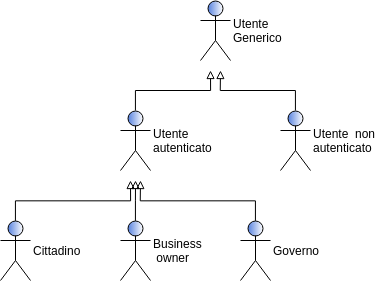
\includegraphics[width=7cm]{res/images/attori_primari.png}
	\centering
	\caption{Gerarchia attori primari}
\end{figure}
\begin{description}[style=nextline]
	\item[Utente Generico]
	Si riferisce ad un utente generico che accede alla piattaforma dal sito web;
	\item[Utente non autenticato]
	Si riferisce ad un utente generico che non ha ancora effettuato l'autenticazione alla piattaforma;
	\item[Utente autenticato]
	Si riferisce ad un utente generico che si è autenticato nel sistema con la procedura di login. Ciò implica che sia in possesso di una chiave pubblica valida sulla rete Ethereum con la quale, precedentemente, ha portato a termine la procedura di autenticazione;
	\item[Cittadino] Si riferisce ad un utente che si è autenticato nel sistema con il ruolo di cliente;
	\item[Azienda] Si riferisce ad un utente che si è autenticato nel sistema con il ruolo di azienda. Le azioni sono eseguite considerando l'azienda come persona giuridica, nonostante le azioni vengano eseguite da un suo rappresentante;
	\item[Governo\glo] Si riferisce ad un utente che si è autenticato al sistema con il ruolo di governo\glo.
\end{description}
\subsubsection{Attori secondari}\begin{description}[style=nextline]
	\item[MetaMask]
	Plug-in per browser che permette di interfacciarsi con la rete Ethereum\glosp e di validare le transazioni con la propria chiave privata.

\end{description}
 
